\documentclass{cekarticle}
\usepackage{color}
\usepackage{amsmath}
\usepackage{amssymb}
\usepackage{array}

\begin{document}

%=============================================================================
% Title page
%=============================================================================

\title{Systems Biology Markup Language (SBML) Level 2 Proposal: Array Features}

\author{Andrew Finney, Victoria Gor, Ben Bornstein, Eric Mjolsness, Hamid Bolouri}

\authoremail{
\begin{minipage}{\textwidth}\centering
afinney@cds.caltech.edu, gor@aig.jpl.nasa.gov, bornstei@aig.jpl.nasa.gov\\Eric.D.Mjolsness@jpl.nasa.gov, hbolouri@cds.caltech.edu
\end{minipage}}

\maketitlepage

%=============================================================================
\section{Introduction}
\label{sec:introduction}
%=============================================================================

This document describes proposed features for inclusion in
Systems Biology Markup Language (SBML) Level 2. This document
describes features enabling the inclusion of arrays of processes,
structures or entities in models.  These features would allow a
model to be assembled from many copies of identical parts.  These
features enable the representation of patterns of connection
amongst array elements.

This document is not a definition of SBML Level 2 or part of it.
This document simply presents various features which could be
incorporated into SBML Level 2 as the Systems Biology community
wishes.  This document is intended for detailed review by that
community and to provoke alternative proposals.  Throughout this
document issues that the authors believe will require further
discussion have been highlighted.

For brevity the text of this document is with reference to SBML
Level 1~\citep{hucka:2001} i.e. features are described in terms
of changes to SBML Level 1.  This document uses UML diagrams in
the same way except that new features are shown in red.

All types proposed in this document will be derived from the
\texttt{SBase} type.

The features described in this document are built upon the
features defined in~\citet{finney:2002c}.

The appendix~\ref{sec:operators} lists all the SBML Level 1
operators with all the operators proposed in this document and in
~\citet{finney:2002c}.

\section{Models}

The proposed structure of the \texttt{Model} type is shown in
figure~\ref{fig:model}. A model would have an optional list of
\texttt{Domain} structures.

\begin{figure}[h]
  \vspace*{8pt}
  \centering
  
\includegraphics[scale = 0.7]{model}
  \caption{The definition of the Model type}
  \label{fig:model}
\end{figure}

\texttt{Domain} structures are described in
section~\ref{sec:domain}.

\section{Domains}
\label{sec:domain}

In this proposal the bounds of an array are separated from an
actual array definition.  Array bounds are defined by these
proposed \texttt{Domain} structures, which are shown in UML form
in figure~\ref{fig:domain}.  A \texttt{Domain} structure consists
of inclusive upper and lower bounds of \texttt{int} type and a
set of symbols which have values over the domain.  The domain
structure simply defines that the symbols in the given set have
all integer values between and including the given bounds.  The
bound values can be negative.  The upper bound must be greater
than the lower bound.

\begin{figure}[h]
  \vspace*{8pt}
  \centering
  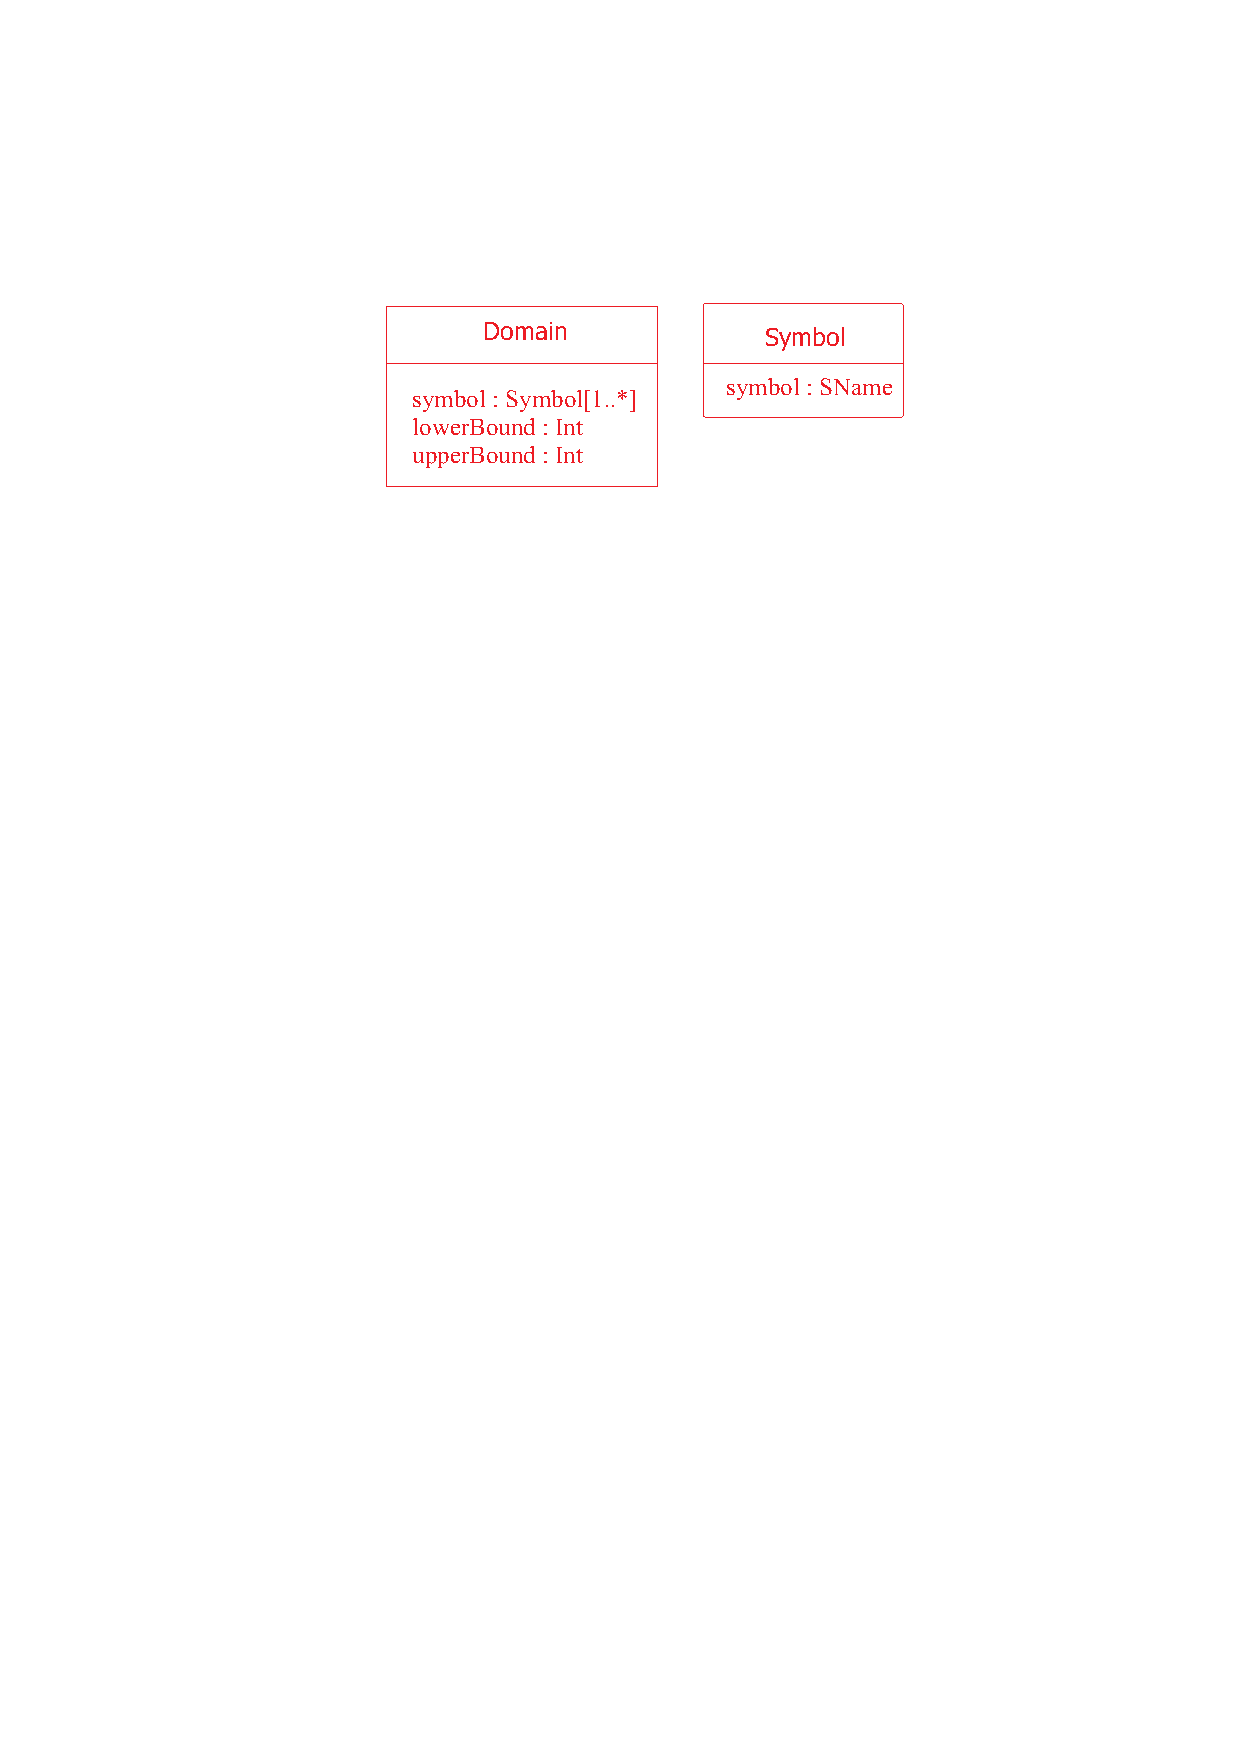
\includegraphics[scale = 0.7]{domain}
  \caption{The definition of the Domain type}
  \label{fig:domain}
\end{figure}

The following example shows a \texttt{Model} structure
incorporating a \texttt{Domain} structure which ranges from -10
through to 10.  The symbols \texttt{x} and \texttt{y} are defined
to have values over the given domain.

\begin{example}
<model name="tissue">
    <listOfDomains>
        <domain upperBound="10" lowerBound="-10">
            <listOfSymbols>
                <symbol name="x"/>
                <symbol name="y"/>
            </listOfSymbols>
        </domain>
    </listOfDomains>
    ...
</model>
\end{example}

\subsection{Constant Symbols and Expressions}
\label{sec:constantExpressions}

The symbol field of a \texttt{Symbol} structure defines a symbol
which can be used in numeric expressions.  The scope of these
symbols is defined in section~\ref{sec:arrays}. Although these
symbol values vary over a domain they are constant for the
duration of a simulation.  These symbols are called
\emph{constant symbols}. It is possible to create expressions
using these symbols. It is possible to distinguish between
constant and dynamic expressions: in a constant expression all
operands and function arguments are either constant symbols or a
constant numeric values.

Constant expressions can then be used in place of most constant
attribute values of type \texttt{double} throughout SBML although
there are limitations on which specific expression they can be
used in, see section~\ref{sec:arrays}. Constant symbols can occur
in any numeric expression, for example a rate equation. As
constant symbols are used in expressions they share the same
namespace as other SBML structures such as species.

\section{Arrays}
\label{sec:arrays}

The core of this proposal is the idea that almost all the
structures in SBML can be defined as arrays as well as single
named objects.  We propose that following SBML types,
\texttt{Specie}, \texttt{Compartment}, \texttt{Reaction},
\texttt{Parameter} and \texttt{Rule} can be defined as arrays of
objects.

To declare and operate on arrays we introduce the \texttt{[]}
array operator, which is similar to the C array operator.  As in
C the array operator is prefixed by a symbol name and should
contain a constant expression.  Several array operators can be
combined to indicate multiple dimensions.   As in C there are 2
uses of the array operator: declaring arrays and accessing array
elements.

\subsection{Array Declaration}

The array operator can be used in the \texttt{name} fields of
\texttt{Specie}, \texttt{Compartment}, \texttt{Reaction} and
\texttt{Parameter} structures and the object reference field of
\texttt{Rule} structures to indicate that the given structure is
an array rather than a single object. All the objects in the
array have the properties described by the structures's
attributes and substructures.

Structures that are declared as arrays share the same namespace
as those structures that represent single objects.

The following SBML fragment shows a \texttt{Compartment}
structure representing a 1 dimensional array.

\begin{example}
<model name="simple">
    <listOfDomains>
        <domain upperBound="9" lowerBound="0">
            <listOfSymbols>
                <symbol name="x"/>
            </listOfSymbols>
        </domain>
    </listOfDomains>
    <listOfCompartments>
        <compartment name="cell[x]"/>
    </listOfCompartments>
    ...
</model>
\end{example}

\subsubsection{Symbol Scope}

Domain symbols used in the expressions contained in array declarations
can be used in attributes of the same structure and sub
structures of that structure.  This is the only place in which
these symbols can be used other than in array declarations.

The following example shows how a symbol can be used in numeric
fields within the symbols scope:

\begin{example}
<model name="ref">
    <listOfDomains>
        <domain upperBound="9" lowerBound="0">
            <listOfSymbols>
                <symbol name="x"/>
            </listOfSymbols>
        </domain>
    </listOfDomains>
    <listOfCompartments>
        <compartment name="cell[x]" volume="x * 0.2" />
    </listOfCompartments>
    ...
</model>
\end{example}

Notice that although constant symbol \texttt{x} varies between 9
and 0 this variance only defines the structure of the model so
that \texttt{x} is not a parameter or variable of any simulation
of the model.

\subsubsection{Simple Sparse Arrays}

Given the scheme described above it is possible to define sparse
arrays. Array elements are only created once for each value of a
domain symbol. The index of a created array element is the result
of the constant expression contained in the array operator. In an
array declaration involving more than one array operator, i.e. an
declaration for a multi-dimensional array, each symbol only runs
over its range once. For example consider the following model:

\begin{example}
<model name="notsimple">
    <listOfDomains>
        <domain upperBound="9" lowerBound="0">
            <listOfSymbols>
                <symbol name="x"/>
                <symbol name="y"/>
            </listOfSymbols>
        </domain>
    </listOfDomains>
    <listOfCompartments>
        <compartment name="cell2D[x][y]"/>
        <compartment name="cellDiagonal[x][x]"/>
    </listOfCompartments>
    ...
</model>
\end{example}

In the model \texttt{notsimple} the array \texttt{cell2D} is square array
containing 100 elements.  \texttt{cellDiagonal} is a 2D array containing
elements only on the diagonal.

The following example creates an array where elements occur at even locations:

\begin{example}
<model name="even">
    <listOfDomains>
        <domain upperBound="9" lowerBound="0">
            <listOfSymbols>
                <symbol name="x"/>
                <symbol name="y"/>
            </listOfSymbols>
        </domain>
    </listOfDomains>
    <listOfCompartments>
        <compartment name="cell2D[2*x][2*y]"/>
    </listOfCompartments>
    ...
</model>
\end{example}

\subsubsection{Declaring arrays of rules}

Declaring arrays of rules is slightly different from the cases
described above. Rule structures don't contain a \texttt{name}
field that declares a new symbol instead they reference another
structure.  When declaring an array of rules the array operator
is used in the object reference field i.e. the \texttt{specie},
\texttt{compartment} and \texttt{name} field for
\texttt{SpecieConcentrationRule}, \texttt{CompartmentVolumeRule}
and \texttt{ParameterRule} structures respectively. The symbol
prefixing the array operator should be an array of the appropriate
type e.g. a specie array for the \texttt{specie} field.  The
expressions enclosed in the array operator in the object
reference field operate in the same way as described above except
that the declaration uses those expressions to link back to the
referenced array.  For example the following model has a rule
applied to an array of species.

\begin{example}
<model name="rules">
    <listOfDomains>
        <domain upperBound="9" lowerBound="0">
            <listOfSymbols>
                <symbol name="x"/>
            </listOfSymbols>
        </domain>
    </listOfDomains>
    ...
    <listOfSpecies>
        <species name="s[x]" initialAmount="0.1"/>
    </listOfSpecies>
    ...
    <listOfRules>
        <specieConcentrationRule specie="s[x]" type="rate" formula="0.1"/>
    </listOfRules>
</model>
\end{example}

As rules do not declare symbols it is possible for more than one
rule to be applied to the same array. For example consider the
following example:

\begin{example}
<model name="rules">
    <listOfDomains>
        <domain upperBound="9" lowerBound="0">
            <listOfSymbols>
                <symbol name="x"/>
            </listOfSymbols>
        </domain>
        <domain upperBound="5" lowerBound="0">
            <listOfSymbols>
                <symbol name="w"/>
            </listOfSymbols>
        </domain>
        <domain upperBound="9" lowerBound="6">
            <listOfSymbols>
                <symbol name="v"/>
            </listOfSymbols>
        </domain>
    </listOfDomains>
    ...
    <listOfSpecies>
        <species name="s[x]" initialAmount="0.1" compartment="cell"/>
    </listOfSpecies>
    ...
    <listOfRules>
        <specieConcentrationRule specie="s[w]" type="rate" formula="0.1"/>
        <specieConcentrationRule specie="s[v]" type="rate" formula="0.2"/>
    </listOfRules>
</model>
\end{example}

\subsubsection{Rules applied to a whole arrays or slices of arrays}

Rules can be defined which apply to the whole of an array, or
slices of arrays, in which the formula expression returns a whole
array value rather than a single value to be inserted into each
array element.  This kind of rule is declared simply by not
applying the array operator to an array symbol, or using the array
slice operator (see section~\ref{sec:placeholder}), in the rule
object reference field.  Whole matrix operators are described in
more detail in section~\ref{sec:math}.  For now assume that we
can, for instance, multiply arrays then consider the example
model:

\begin{example}
<model name="rules">
    <listOfDomains>
        <domain upperBound="9" lowerBound="0">
            <listOfSymbols>
                <symbol name="x"/>
            </listOfSymbols>
        </domain>
    </listOfDomains>
    ...
    <listOfSpecies>
        <species name="s1[x]" initialAmount="0.1"/>
        <species name="s2[x]" initialAmount="0.2"/>
    </listOfSpecies>
    ...
    <listOfRules>
        <specieConcentrationRule specie="s1" type="rate" formula="s1 * s2"/>
    </listOfRules>
</model>
\end{example}

The rule for \texttt{s1} defines that the rate of change of the
values of the array of \texttt{s1} is the product of the matrices
\texttt{s1} and \texttt{s2}.

\subsubsection{Issues}
\begin{itemize}
\item
It is possible to avoid the use of the array operator in the name
field for array declarations and instead use XML structures
instead.  This would mean that a SBML parser would avoid having
to parse the content of the \texttt{name} field.  For example the
following model
\begin{example}
<model name="simple">
    <listOfDomains>
        <domain upperBound="9" lowerBound="0">
            <listOfSymbols>
                <symbol name="x"/>
            </listOfSymbols>
        </domain>
    </listOfDomains>
    <listOfCompartments>
        <compartment name="cell[x]"/>
    </listOfCompartments>
    ...
</model>
\end{example}
can be recast as:
\begin{example}
<model name="simple">
    <listOfDomains>
        <domain upperBound="9" lowerBound="0">
            <listOfSymbols>
                <symbol name="x"/>
            </listOfSymbols>
        </domain>
    </listOfDomains>
    <listOfCompartments>
        <compartment name="cell">
            <listOfDimensions>
                <dimension formula="x"/>
            </listOfDimensions>
        </compartment>
    </listOfCompartments>
    ...
</model>
\end{example}

\item
We could eliminate simple sparse arrays by restricting the
expressions inside array operators used in declarations to be
just symbols rather than constant expressions and by forcing the
symbol in each dimension to be unique within the declaration.
\end{itemize}

\subsection{Array Element Reference}
In this section mechanisms for accessing specific elements of an
array are described. In numeric expressions the array operator is
syntactically equivalent to a function call and returns the value
of the indexed array element. The array operator can also be used
in any field which refers to a \texttt{Specie},
\texttt{Compartment}, \texttt{Reaction} or \texttt{Parameter} by
name, for example the \texttt{specie} field on a
\texttt{SpecieReference} structure can contain an array operator
instead of an \texttt{SName} type.  In these fields the array
operator is used to refer to a specific element.

The `array' operand of an array operator must be the name of a
structure which has been declared as an array. An array operator,
when applied to an array consisting of $n$ dimensions, results in
an array of $n-1$ dimensions and if $n$ is 1 then the result is a
single object, for example given an array declared as $a[x][y]$
(a 2 dimensional array) then $a[1]$ is a one dimensional array
and $a[1][1]$ refers to a single element.

We can use the array operator to create an array of species
distributed across an array of compartments:
\begin{example}
<model name="ref">
    <listOfDomains>
        <domain upperBound="9" lowerBound="0">
            <listOfSymbols>
                <symbol name="x"/>
            </listOfSymbols>
        </domain>
    </listOfDomains>
    <listOfCompartments>
        <compartment name="cell[x]"/>
    </listOfCompartments>
    <listOfSpecies>
        <species name="s[x]" compartment="cell[x]"/>
    </listOfSpecies>
    ...
</model>
\end{example}
In this example each species array element is placed in a
corresponding compartment.

\subsubsection{Restriction}
We suggest that for SBML Level 2, the index operand to an array
operator be restricted to being a constant expression.

\subsubsection{Issue}
We could use a new element to reference elements from an object
reference field instead of putting the array operator inside the
object reference fields. For example the above example can be
re-formulated as:
\begin{example}
<model name="ref">
    <listOfDomains>
        <domain upperBound="9" lowerBound="0">
            <listOfSymbols>
                <symbol name="x"/>
            </listOfSymbols>
        </domain>
    </listOfDomains>
    <listOfCompartments>
        <compartment name="cell">
            <listOfDimensions>
                <dimension formula="x"/>
            </listOfDimensions>
        </compartment>
    </listOfCompartments>
    <listOfSpecies>
        <species name="s" compartment="cell">
            <listOfDimensions>
                <dimension formula="x"/>
            </listOfDimensions>
            <listOfCompartmentElementReferences>
                <dimension formula="x"/>
            </listOfCompartmentElementReferences>
        </species>
    </listOfSpecies>
    ...
</model>

\end{example}
We will still need to be able to parse the array operator in
numeric expressions.

\subsubsection{Example of using element references in both numeric and object reference fields}
The following example shows how the array operator can be used in
a numeric expression.

\begin{example}
<model name="ref">
    <listOfDomains>
        <domain upperBound="9" lowerBound="0">
            <listOfSymbols>
                <symbol name="x"/>
            </listOfSymbols>
        </domain>
    </listOfDomains>
    <listOfCompartments>
        <compartment name="cell"/>
    </listOfCompartments>
    <listOfSpecies>
        <species name="s1[x]" compartment="cell"/>
        <species name="s2[x]" compartment="cell"/>
    </listOfSpecies>
    <listOfReactions>
        <reaction name="r[x]">
            <listOfReactants>
                <specieReference specie="s1[x]"/>
            </listOfReactants>
            <listOfProducts>
                <specieReference specie="s2[x]"/>
            </listofProducts>
            <kineticLaw formula="s1[x] * 0.1"/>
        </reaction>
    </listOfReactions>
</model>
\end{example}

\subsubsection{Referring to elements of a sparse array}

The index operand to an array operator must refer to an element
which exists in an array.  For example the following model is
inconsistent:

\begin{example}
<model name="ref">
    <listOfDomains>
        <domain upperBound="9" lowerBound="0">
            <listOfSymbols>
                <symbol name="x"/>
            </listOfSymbols>
        </domain>
    </listOfDomains>
    <listOfCompartments>
        <compartment name="cell[x * 2]"/>
    </listOfCompartments>
    <listOfSpecies>
        <species name="s" compartment="cell[1]"/>
    </listOfSpecies>
    ...
</model>
\end{example}

The element \texttt{cell[1]} has not been declared.

\section{Conditional Sparse Arrays and Connections}

\subsection{Conditional Sparse Arrays}

In practice arrays are not very useful for modeling unless its
possible to describe connection schemes between elements of the
arrays.  For example if one creates a model of a tissue of cells
as an array of compartments then the model doesn't become
interesting until the interactions between the cells are
incorporated.  This section begins the process of proposing
structures which allow interconnection schemes to be defined.

In this proposal the structures \texttt{Specie},
\texttt{Compartment}, \texttt{Reaction} and \texttt{Parameter} and
\texttt{Rule} include an additional \texttt{elementExists}
field.  This field should only occur when the structure is
declared as an array.  \texttt{elementExists} contains a constant
expression which defines whether an array element actually occurs
at a given position in the array.  This expression is
conditional, which means that a zero value (false) implies that
the element won't occur and a non-zero value (true) implies that
an element will occur (conditional expressions are described in
more detail in~\citet{finney:2002c}).

The default value of \texttt{elementExists}, 1, ensures that by
default the shape of the array specification is determined just
by the array operator alone.

Apart from the \texttt{elementExists} field, constant
symbols only have values for those elements that exist in the
array in which they are declared.

The index operand to an array operator must refer to a an element
which exists in the array.  This means that the index must be a
value to which the \texttt{elementExists} expression returns a
non-zero value.

\subsubsection{Restriction}

We propose that for SBML Level 2 that \texttt{elementExists}
values are constant expressions.

\subsubsection{Issue}

To enable dynamic structures in SBML we could allow the
\texttt{elementExists} expression to be dynamic. This would allow
the model to change dynamically during the simulation.  Perhaps
other more explicit dynamic restructuring of a model should be
considered in SBML.

\subsection{Conditional Sparse Array Example}
\label{sec:sparseeg}

The following example shows a proposed structure for triangular
arrays where the maximum \texttt{y} index is equal to the
\texttt{x} index.

\begin{example}
<model name="starfish">
    <listOfDomains>
        <domain upperBound="9" lowerBound="0"/>
            <listOfSymbols>
                <symbol name="x"/>
                <symbol name="y"/>
            </listOfSymbols>
        </domain>
    </listOfDomains>
    <compartment name="cell[x][y]" elementExists="y <= x">
    ...
</model>
\end{example}

\subsection{Using Conditional Sparse Arrays to Represent Connection schemes}
\label{sec:connections}

We can use a proposed sparse array to represent the connections
between elements of another array.  This is shown in the
following example, in which \texttt{grid} is a 2 dimensional
array of compartments and, \texttt{connections} is a sparse 4
dimensional array of reactions between elements of \texttt{grid}.
\texttt{connections} contains adjacent array elements for all
pairs of co-ordinates (over the \texttt{x} and \texttt{y}
domains) where the co-ordinates are exactly one array element
away from each other.

\begin{example}
<model name="tissue">
    <listOfDomains>
        <domain upperBound="9" lowerBound="0">
            <listOfSymbols>
                <symbol name="x"/>
                <symbol name="y"/>
                <symbol name="x1"/>
                <symbol name="x2"/>
                <symbol name="y1"/>
                <symbol name="y2"/>
            </listOfSymbols>
        </domain>
    </listOfDomains>
    <listOfCompartments>
        <compartment name="grid[x][y]"/>
    </listOfCompartments>
    <listOfSpecies>
        <species name="s[x][y]" initialAmount="0.1" compartment="grid[x][y]"/>
    </listOfSpecies>
    <listOfReactions>
        <reaction
                name="connections[x1][y1][x2][y2]"
                elementExists="abs(x2 - x1) == 1 || abs(y2 - y1) == 1">

            <listOfReactants>
                <specieReference specie="s[x1][y1]"/>
            </listOfReactants>
            <listOfProducts>
                <specieReference specie="s[x2][y2]"/>
            </listOfProducts>
            <kineticLaw formula="s[x1][y1] * 0.1"/>

        </reaction>
    </listOfReactions>
</model>
\end{example}

The \texttt{connections} specification is bidirectional: for every
pair of adjacent \texttt{grid} co-ordinates there are a pair of
elements. \texttt{connections} can be simplified and made
unidirectional by changing the \texttt{elementExists} expression
to:
\begin{example}
x2 - x1 == 1 || y2 - y1 == 1
\end{example}
In this case the connections only run from bottom to top and left
to right.

Often its convenient to use \texttt{Function} structures in the
\texttt{elementExists} field. The following example, uses a
\texttt{Function} structure to define an more explicit connection
scheme.

\begin{example}
<model name="spotty">
    <listOfFunctions>
        <function name="explicit"
            formula="(x==1 && y==1) || (x==3 && y==3) || (x==0 && y==9)">
            <listOfArguments>
                <argument name="x"/>
                <argument name="y"/>
            </listOfArguments>
        </function>
    </listOfFunctions>
    <listOfDomains>
        <domain upperBound="9" lowerBound="0">
            <symbol name="a"/>
            <symbol name="b"/>
        </domain>
    </listOfDomains>
    ...
    <listOfReactions>
        <reaction name="spots[a][b]" elementExists="explicit(a, b)">
            ...
        </reaction>
    </listOfReactions>
</model>
\end{example}

\section{Simplified Array Structures for Related Objects}

It is possible to incorporate a simplified mechanism for creating
species, compartment and parameter arrays and for referencing the
elements of those arrays.

\subsection{Implied Species Arrays}
\label{sec:impliedarrays}

In this proposal the \texttt{compartment} field of a
\texttt{Specie} structure can consist of a name of an array of
compartments, without an array operator. This kind of structure
represents an array of species with the same specification as the
given compartment array.  Each element of the specie array is
located in a corresponding compartment element.  The specie array
doesn't have to be explicitly declared.

For example given
\begin{example}
<domain lowerBound="0" upperBound="9"/>
    <listOfSymbols>
        <symbol name="x"/>
        <symbol name="y"/>
    </listOfSymbols>
</domain>
...
<compartment name="cell[x][y]"/>
\end{example}
the structure
\begin{example}
<specie name="s[x][y]" compartment="cell[x][y]" initialAmount="x == 0 ? 1e-10 : 0"/>
\end{example}
can be replaced with the equivalent structure
\begin{example}
<specie name="s" compartment="cell" initialAmount="x == 0 ? 1e-10 : 0"/>
\end{example}

It is important to note that in the second case the symbol
\texttt{x} is in scope even though it doesn't appear in the
\texttt{specie} structure directly.  For the purposes of this
document, arrays declared using form of the second case are called
implied arrays. Elements of implied arrays created this way can
be referenced as described in previous sections.

If the specie \texttt{name} field includes an array operator in this kind of
structure the resulting specie array created is the combination
of the compartment and species arrays.  For example the following structures defines a 3
dimension array of species where 2 dimensions are mapped across a
grid of compartments:
\begin{example}
<listOfDomains>
    <domain lowerBound="0" upperBound="9"/>
        <listOfSymbols>
            <symbol name="x"/>
            <symbol name="y"/>
        </listOfSymbols>
    </domain>
    <domain lowerBound="0" upperBound="5"/>
        <listOfSymbols>
            <symbol name="i"/>
        </listOfSymbols>
    </domain>
<listOfDomains>
...
<compartment name="cell[x][y]"/>
...
<specie name="ss[i]" compartment="cell" initialAmount="0"/>
\end{example}

\subsection{Implied Compartment Arrays}

In SBML Level 1 it is possible to specify nested compartments.
For example the fragment:

\begin{example}
<listOfCompartments>
    <compartment name="a">
    <compartment name="b" outside="a">
</listOfCompartments>
\end{example}

Defines a compartment \texttt{b} which is enclosed by \texttt{a}.

We can extend the structure defined in section~\ref{sec:impliedarrays} to cover
nested compartments.

For example given

\begin{example}
<domain lowerBound="0" upperBound="5"/>
    <listOfSymbols>
        <symbol name="i"/>
    </listOfSymbols>
</domain>
\end{example}

then

\begin{example}
<listOfCompartments>
    <compartment name="a[i]"/>
    <compartment name="b" outside="a"/>
</listOfCompartments>
\end{example}

is equivalent to

\begin{example}
<listOfCompartments>
    <compartment name="a[i]"/>
    <compartment name="b[i]" outside="a[i]"/>
</listOfCompartments>
\end{example}

\subsection{Implied Parameter Arrays}

We can apply the above concept to parameters if we introduce a
new \texttt{SName} field, \texttt{foreach}, to the parameter
structure. This field allows us to reference any other symbol
from this structure and thus attach a parameter to each element
of the referenced array.

For example the model:
\begin{example}
<listOfDomains>
    <domain lowerBound="0" upperBound="5"/>
        <listOfSymbols>
            <symbol name="i"/>
        </listOfSymbols>
    </domain>
<listOfDomains>
...
<compartment name="cell[i]"/>
...
<parameter name="p" foreach="cell" value="0"/>
...
\end{example}
is equivalent to
\begin{example}
<listOfDomains>
    <domain lowerBound="0" upperBound="5"/>
        <listOfSymbols>
            <symbol name="i"/>
        </listOfSymbols>
    </domain>
<listOfDomains>
...
<compartment name="cell[i]"/>
...
<parameter name="p[i]" value="0"/>
...
\end{example}

\subsection{Referencing nested array elements}

To compliment the above simplification we introduce a new
operator `\texttt{.}' which has precedence between function
operators and the '\texttt{*}' and `\texttt{/}' operators. The
left hand operand of this operator is an expression representing
a containing object. The right hand side is a symbol representing
an object within the left hand object.

If the object on the left hand side is an element of an
array then it is assumed that the right hand object is also an array
distributed across the elements of the array. In which case
the `\texttt{.}' operator returns the element
corresponding to the left hand array element.

Consider the following model:

\begin{example}
<model>
    <listOfDomains>
        <domain lowerBound="0" upperBound="5"/>
            <listOfSymbols>
                <symbol name="i"/>
            </listOfSymbols>
        </domain>
    <listOfDomains>
    <listOfCompartments>
        <compartment name="cell[i]"/>
    </listOfCompartments>
    <listOfSpecies>
        <species name="s1[i]" compartment="cell[i]"/>
        <species name="s2[i]" compartment="cell[i]"/>
    </listOfSpecies>
    <reaction name="j[i]">
        <listOfReactants>
            <specieReference specie="s1[i]" stoichiometry="1"/>
        </listOfReactants>
        <listOfProducts>
            <specieReference specie="s2[i]" stoichiometry="1"/>
        </listOfProducts>
        <kineticLaw formula="s1[i] * 5"/>
    </reaction>
</model>
\end{example}
This can be written as
\begin{example}
<model>
    <listOfDomains>
        <domain lowerBound="0" upperBound="5"/>
            <listOfSymbols>
                <symbol name="i"/>
            </listOfSymbols>
        </domain>
    <listOfDomains>
    <listOfCompartments>
        <compartment name="cell[i]"/>
    </listOfCompartments>
    <listOfSpecies>
        <species name="s1" compartment="cell"/>
        <species name="s2" compartment="cell"/>
    </listOfSpecies>
    <reaction name="r[i]">
        <listOfReactants>
            <specieReference specie="cell[i].s1" stoichiometry="1"/>
        </listOfReactants>
        <listOfProducts>
            <specieReference specie="cell[i].s2" stoichiometry="1"/>
        </listOfProducts>
        <kineticLaw formula="cell[i].s1 * 5"/>
    </reaction>
</model>
\end{example}

The `\texttt{.}' operator can be used with arrays of species which
have more dimensions than the compartments in which they are
located. For example consider the following model:
\begin{example}
<model>
    <listOfDomains>
        <domain lowerBound="0" upperBound="5"/>
            <listOfSymbols>
                <symbol name="i"/>
            </listOfSymbols>
        </domain>
        <domain lowerBound="0" upperBound="10"/>
            <listOfSymbols>
                <symbol name="j"/>
            </listOfSymbols>
        </domain>
    <listOfDomains>
    <listOfCompartments>
        <compartment name="cell[i]"/>
    </listOfCompartments>
    <listOfSpecies>
        <species name="s1[j]" compartment="cell"/>
        <species name="s2[j]" compartment="cell"/>
    </listOfSpecies>
    <reaction name="r[i][j]">
        <listOfReactants>
            <specieReference specie="cell[i].s1[j]" stoichiometry="1"/>
        </listOfReactants>
        <listOfProducts>
            <specieReference specie="cell[i].s2[j]" stoichiometry="1"/>
        </listOfProducts>
        <kineticLaw formula="cell[i].s1[j] * 5"/>
    </reaction>
</model>
\end{example}

It is possible to create a model with more than one level of nesting.
For example:

\begin{example}
<model>
    <listOfDomains>
        <domain lowerBound="0" upperBound="5">
            <listOfSymbols>
                <symbol name="i"/>
            </listOfSymbols>
        </domain>
    </listOfDomains>
    <listOfCompartments>
        <compartment name="a[i]"/>
        <compartment name="b" outside="a"/>
    </listOfCompartments>
    </listOfSpecies>
        <specie name="s1" compartment="b" initialAmount="0.1"/>
        <specie name="s2" compartment="b" initialAmount="0.1"/>
    </listOfSpecies>
    <listOfReactions>
        <reaction name="r[i]">
            <listOfReactions>
                <specieReference specie="a[i].b.s1"/>
            </listOfReactions>
            <listOfProducts>
                <specieReference specie="a[i].b.s2"/>
            </listOfProducts>
        </reaction>
    </listOfReactions>
</model>
\end{example}
This array proposal does not change any of the existing namespace
rules of SBML: for example species located in different compartments cannot
have the same name.

\subsection{Issues}

\begin{itemize}
\item
The simplified structures and the `\texttt{.}' operator
described in this section are redundant.  Should they be
incorporated into SBML Level 2?
\item
The above definition implies that elements of an array defined using the implied forms
described in this section can be referenced by either the `.' operator or indexing the array directly.
For example given:
\begin{example}
<listOfDomains>
    <domain upperBound="0" lowerBound="9">
        <symbol name="x"/>
    </domain>
    <domain upperBound="0" lowerBound="3">
        <symbol name="y"/>
    </domain>
</listOfDomains>
<listOfCompartments>
    <compartment name="cell[x]"/>
</listOfCompartments>
<listOfSpecies>
    <specie name="s[y]" compartment="cell"/>
</listOfSpecies>
\end{example}
elements of \texttt{s} can be referenced in two equivalent ways:
\begin{example}
<specieReference specie="s[x][y]"/>
\end{example}
or
\begin{example}
<specieReference specie="cell[x].s[y]"/>
\end{example}

Is this a good idea?

\item
Is it a good idea that the symbols used in a implied array declaration
can include those used in the enclosing structure and not only
those using in the immediate enclosed structure?
Note the following is possible:

\begin{example}
...
<domain lowerBound="0" upperBound="9"/>
    <listOfSymbols>
        <symbol name="x"/>
        <symbol name="y"/>
    </listOfSymbols>
</domain>
...
<compartment name="cell[x][y]"/>
...
<specie name="s" compartment="cell" initialAmount="x == 0 ? 1e-10 : 0"/>
...
\end{example}

\item
Following on from previous issue, the same domain symbol
appearing twice in the same nested structure can have confusing
results. For example given:
\begin{example}
<listOfDomains>
    <domain upperBound="0" lowerBound="9">
        <symbol name="x"/>
    </domain>
</listOfDomains>
<listOfCompartments>
    <compartment name="cell[x]"/>
</listOfCompartments>
\end{example}
then
\begin{example}
<listOfSpecies>
    <specie name="s[x]" compartment="cell"/>
</listOfSpecies>
\end{example}
is equivalent to
\begin{example}
<listOfSpecies>
    <specie name="s[x][x]" compartment="cell[x]"/>
</listOfSpecies>
\end{example}

This means that a sparse array of species has been created.

Should a parser detect this as an error or simply warn the user?
This is this another good reason for modifying the
scope of the symbols declared in the enclosing structure?
\end{itemize}

\section{Array Math}
\label{sec:math}

This section describes a set of proposed operators and functions
that can be performed on arrays in formulas.

\subsection{Operators}

We propose that a subset of the matrix operators defined in
MATLAB~\citep{matlab:1998} are incorporated into SBML. An initial
subset for Level 2 might be: \texttt{+}, \texttt{-}, \texttt{*},
\texttt{./}, \texttt{.*}, \verb+.^+ and \texttt{'}.
Appendix~\ref{sec:operators} shows how these operators are
integrated into SBML.

\subsection{\texttt{:} Array Index Placeholder}
\label{sec:placeholder}

In this proposal the character `\texttt{:}' can be used as a
place holder for array indices.  The result of using such a place
holder is an array which is a slice of the original array. The
precise definition of this operation is taken from
MATLAB~\citep{matlab:1998}.  For example given a 2 dimensional
array \texttt{x} the expression \texttt{x[:][i]} returns the 1
dimensional array of the ith row of the array.

SBML uses the \texttt{:} operation in combination with the 'C'
language notation for arrays so that if we consider a two
dimensional array, \texttt{a}, then \texttt{a[:][:]} is
equivalent to \texttt{a} and \texttt{a[i][:]} is equivalent to
\texttt{a[i]}.

\subsection{Built-In Array Functions}

We propose the following built-in functions for matrix math:

\begin{example}
sum(array)
\end{example}

This function returns the sum of all the elements of the given array

\begin{example}
sum(expression, symbol1, lowerBound1, upperBound1,...
    symboln, lowerBoundn, upperBoundn)
\end{example}
This function's arguments consist of an expression followed by a
sequence of triples.  The triples sequence consist of 1 or more
triples. Each triple consists of a symbol, which is a new
constant integer symbol (i.e. not an expression) sharing the same
namespace as species, compartment etc plus an upper and lower
bound.  The symbols only have scope within following the following
arguments.  The upper and lower bounds are truncated to integers.

This function simply runs through all the possible symbol values
between the computed bounds.  For each set of symbol values the
final expression is evaluated.  The function returns the sum of
these final expression values.

\begin{example}
sumOverDomain(expression, domainSymbol1, ... domainSymboln)
\end{example}
This function's arguments consist of an expression followed by a
sequence of domain symbols.  The domain symbols only have scope
in the expression argument.  The domain symbols cannot be any of
the domain symbols already used in the scope outside the function
call.

This function simply runs through all the possible symbol values
with the domains.  For each set of symbol values the final
expression is evaluated.  The function returns the sum of these
final expression values.

\begin{example}
product(array)
\end{example}
This function returns the product of all the elements of the
given array

\begin{example}
product(expression, symbol1, lowerBound1, upperBound1,...
    symboln, lowerBoundn, upperBoundn)
\end{example}
Similar to the multiple argument \texttt{sum} function: the only
difference is that \texttt{product} returns the product of the final
expression values.

\begin{example}
productOverDomain(expression, domainSymbol1, domainSymboln)
\end{example}
Similar to the multiple argument \texttt{sumOverDomain} function: the only
difference is that \texttt{product} returns the product of the final
expression values.

\begin{example}
map(function, array)
\end{example}
returns the array which results from the application of
\texttt{function} to all the elements of the given array.
\texttt{function} is a function name only.  The corresponding
function will take a single argument.

\begin{example}
reduce(function, array, startValue)
reduce(function, array)
\end{example}
This function computes a value $x$ through the application of a
function \texttt{function} to elements of the array
\texttt{array}.  The initial value of $x$ is
\texttt{startValue}.  \texttt{function} takes two arguments: the
current value of $x$ and the next element in the array.
\texttt{function} then returns the new value of $x$.
The default value of \texttt{startValue} is zero.

For example given the following structure
\begin{example}
<function name="plus" formula="a + b">
    <listOfArguments>
        <argument name="a"/>
        <argument name="b"/>
    </listOfArguments>
</function>
\end{example}
then the expression
\begin{example}
reduce(plus, s)
\end{example}
is equivalent to
\begin{example}
sum(s)
\end{example}

In more complex functions the order in which the array elements
are applied to the function is significant.  \texttt{reduce} is
computed as a series of nested loops in which the first dimension
forms the outermost loop and the last dimension forms the
innermost loop.

\begin{example}
argmin(expression, symbol)
\end{example}

returns the potential value of previously declared
\texttt{symbol} which clauses \texttt{expression} to return the
minimum value. \texttt{argmin} returns a value but doesn't change
\texttt{symbol}.  \texttt{symbol} can be a scalar or array value.
When \texttt{symbol} is an array then the set of values that
minimize \texttt{expression} is returned.

\begin{example}
argmax(expression, symbol)
\end{example}

Similar to \texttt{argmin} except that the function returns the
value that a maximizes \texttt{expression}.

\subsection{Issues}
\begin{itemize}
\item Some of the above matrix functions are redundant should they be included in SBML?
\item Given that \texttt{argmin} and \texttt{argmax} can't be mapped to SBML Level 1
should they be included in Level 2?  If yes should they be part
of a separate package (called \texttt{optimization})?
\end{itemize}

\section{Complex Example using Array Math}

The following SBML Level 2 example is the complete model which
describes an epithelium consisting of 9 cells with 3 species
inside each cell \texttt{cell[ic].ss[is]}, and the dynamic
development of this epithelium. The species inside each cell
interact with each other and with the species of the neighboring
cells according to a single \texttt{specieConcentrationRule}.
Parameters \texttt{h}, \texttt{lambda}, \texttt{tau},
\texttt{Tin}, \texttt{TOne}, \texttt{Tout} and \texttt{TTwo} are
parameters for the \texttt{specieConcentrationRule} and they
describe how neighboring species interact and develop.

Each cell is allowed to move in 2-dimensional space. To implement
that, each cell has 2-dimensional array of coordinates (an
implied parameter array), associated with it
\verb+cell[I].crd[i_crd]+. Initially, the cells are placed on
two-dimensional (3x3) grid. Cell positions are allowed to change,
and dynamic cell positions are determined from by the
\texttt{parameterRule} for \texttt{crd}. Obviously, once cell
positions change, the neighboring relationships change also. The
list of current neighbors for each cell is determined in function
\texttt{CM} (\texttt{CM} stands for Connection Matrix). This
function returns 1 if given coordinates of two cells indicate
that cells are neighbors (that is cells are connected), and it
returns 0 otherwise. Each pair of cells is considered.

Also involved in cell positioning are the masses of the cells
\texttt{parameter name="mass"} and the connection strengths
\verb+parameter name="CS[i_cnt][j_cnt]"+ between the cells.
Masses of the cells are initially set to 1 and are dynamically
changing according to \texttt{parameterRule name="mass[ic]"}.
Connection strengths are dynamic as well, they depend on initial
equilibrium distance between two cells
\verb+init_eq_dist[i_cnt][j_cnt]+ and on current masses of these
cells. (Remember, function CM determines if two cells are
connected or not). The initial equilibrium distance
\verb+init_eq_dist[i_cnt][j_cnt]+ is a static parameter. No
\texttt{parameterRule} for it exists. This parameter is used to
store the \emph{initial} equilibrium distance between two cells
(as defined by formula for \texttt{value} of this parameter). And
the initial equilibrium distances together with dynamic masses
are used to calculate dynamic connection strength between two
cells in developmental simulations.

This model fully describes the epithelium at initial time, and
all the processes which are needed to calculate the epithelium
condition at any future time.

The SBML Level 2 representation of this model is as follows:

\begin{example}
<?xml version="1.0" encoding="UTF-8"?>
<sbml xmlns="http://www.sbml.org/sbml/level2" version="1" level="2">
<model name="GRN_Equations">

    <listOfFunctions>
        <function name="CM"
            formula=
                "abs(x2-x1) <= 0.2 && abs(y2-y1) <= 0.2 && ( (x2 != x1) || (y2!=y1) )">
            <listOfArguments>
                <argument name="x1"/>
                <argument name="y1"/>
                <argument name="x2"/>
                <argument name="y2"/>
            </listOfArguments>
        </function>
        <function name="sigmoid" formula = "0.5* (1.0+ (x/sqrt(1.0+x*x)))">
            <listOfArguments>
                <argument name="x"/>
            </listOfArguments>
        </function>
    </listOfFunctions>


    <listOfDomains>
      <domain upperBound="8" lowerBound="0">
        <listOfSymbols>
          <symbol name="ic"/>
          <symbol name="I"/>
          <symbol name="K"/>
          <symbol name="i_cnt"/>
          <symbol name="j_cnt"/>
        </listOfSymbols>
      </domain>

      <domain upperBound="2" lowerBound="0">
        <listOfSymbols>
          <symbol name="is"/>
          <symbol name="js"/>
          <symbol name="J"/>
          <symbol name="L"/>
        </listOfSymbols>
      </domain>

      <domain upperBound="2" lowerBound="1">
        <listOfSymbols>
          <symbol name="i_crd"/>
        </listOfSymbols>
      </domain>
    </listOfDomains>

    <listOfCompartments>
      <compartment name="cell[ic]"/>
    </listOfCompartments>

    <listOfSpecies>
      <specie name="ss[is]" compartment="cell" initialAmount="0"/>
    </listOfSpecies>

    <listOfParameters>
      <parameter name="h[is]"        value="1"/>
      <parameter name="lambda[is]"   value="1"/>
      <parameter name="tau[is]"      value="1"/>
      <parameter name="Tin[is][js]"  value="1"/>
      <parameter name="TOne[is][js]" value="1"/>
      <parameter name="Tout[is][js]" value="1"/>
      <parameter name="TTwo[is][js]" value="1"/>
      <parameter name="CS[i_cnt][j_cnt]" value="0"/>
      <parameter name="crd[i_crd]" foreach="cell"
                 value="i_crd == 1 ?
                            (ic div 3 + 1) * 0.1 :
                            (ic mod 3 + 1) * 0.1"/>

      <parameter name="mass" foreach="cell" value="1"/>
      <parameter name="init_eq_dist[i_cnt][j_cnt]"
                 value="( (cell[i_cnt].crd[1]-cell[j_cnt].crd[1])^2 +
                          (cell[i_cnt].crd[2]-cell[j_cnt].crd[2])^2 ) / 2"/>
    </listOfParameters>

    <listOfRules>
        <specieConcentrationRule specie="cell[ic].ss[is]" type="rate"
            formula = "(
                      (-lambda[is]*cell[ic].ss[is]) +
                      sigmoid(
                        h[is] +
sumOverDomain(cell[ic].ss[L]*Tin[is][L], L) +
sumOverDomain(CM(cell[ic].crd[1], cell[ic].crd[2], cell[K].crd[1], cell[K].crd[2]) *
                sumOverDomain(cell[K].ss[L] * Tout[is][L], L), K) +

sumOverDomain(CM(cell[ic].crd[1], cell[ic].crd[2], cell[K].crd[1], cell[K].crd[2]) *
                 sumOverDomain(
                               cell[K].ss[I]  *
                               cell[ic].ss[I] *
                               TOne[J][is]    *
                               TTwo[is][J]),
                               I,
                               J)
                        )
                     ,K) / tau[is]" />

        <parameterRule name="mass[ic]"
                       formula="sumOverDomain(cell[ic].ss[L], L)+1"/>

        <parameterRule name="CS[i_cnt][j_cnt]"
                       formula="init_eq_dist[i_cnt][j_cnt] *( mass[i_cnt]^-3+
                                                              mass[j_cnt]^-3)"/>
        <parameterRule name="crd"
                       formula="
                       argmin(1/2 *
                         sumOverDomain(
                           CM(cell[I].crd[1],cell[I].crd[2],cell[J].crd[1],cell
[J].crd[2]) * ( (((cell[I].crd[1]-cell[J].crd[1])^2 +
(cell[I].crd[2]-cell[J].crd[2])^2)^-2)-CS[I][J])^2, I, J), crd )"/>

    </listOfRules>
</model>
</sbml>

\end{example}

This model doesn't contain any reactions.  We're assuming that
SBML Level 2 will allow models to contain no reactions.

\section{Example: the community effect in developmental gene regulation}

This section contains an example model of the community effect in
developmental gene regulation~\citep{gurdon:1988}. The model basically contains a
high abstracted model of gene expression for a single gene as follows:

\begin{equation*}
  \begin{array}{@{}ccc@{}}
    ubiq & \underrightarrow{v_{mu} ubiq} & waste \\ \\[-4pt]
    mRNA & \underrightarrow{k_{dm} mRNA} & waste \\ \\[-4pt]
    p & \underrightarrow{k_{dp} p} & waste \\ \\[-4pt]
    mat & \underrightarrow{v_i} & ubiq \\ \\[-4pt]
    mat & \underrightarrow{\frac{k_t ubiq}{k_{mu} + ubiq}} & mRNA \\ \\[-4pt]
    mat & \underrightarrow{\frac{k_s mRNA}{k_{mu} + mRNA}} & p
  \end{array}
\end{equation*}

where $ubiq$ is a transcription factor, $p$ is the gene product,
$mat$ represents the material used to construct active species and
$waste$ represents the material produced by the degradation of
active species.  Both $mat$ and $waste$ are modeled as boundary
conditions.

This model is applied to a rectangular array of compartments. The
model contains a positive feedback loop between adjacent cells by
enabling the gene product of an adjacent cell to be a
transcription factor of the gene in the current cell. Thus the
feedback loop is completed by the following reaction for every
pair of adjacent cells $(a,b)$:

\begin{equation*}
  \begin{array}{@{}ccc@{}}
    mat_a & \underrightarrow{\frac{k_r p_b}{k_mr + p_b}} & mRNA_a
  \end{array}
\end{equation*}

where adjacent simply means cells above, below left and right of
the current cell.

The SBML form of this model is as follows:

\begin{example}
<?xml version="1.0" encoding="UTF-8"?>
<sbml xmlns="http://www.sbml.org/sbml/level2" version="1" level="2">
<model name="community_effect">
    <listOfDomains>
        <domain upperBound = "9" lowerBound = "0">
            <symbol name="x"/>
            <symbol name="x1"/>
            <symbol name="x2"/>
        </domain>
        <domain upperBound = "5" lowerBound = "0">
            <symbol name="y"/>
            <symbol name="y1"/>
            <symbol name="y2"/>
        </domain>
    </listOfDomains>
    <listOfCompartments>
        <compartment name="cell[x][y]"/>
    </listOfCompartments>
    <listOfSpecies>
        <specie name="mat" compartment="cell" boundaryCondition="true" initialAmount="1.0"/>
        <specie name="waste" compartment="cell" boundaryCondition="true" initialAmount="1.0"/>
        <specie name="ubiq" compartment="cell" initialAmount="0"/>
        <specie name="mRNA" compartment="cell" initialAmount="0"/>
        <specie name="p" compartment="cell" initialAmount="0"/>
    </listOfSpecies>
    <listOfParameters>
        <parameter name="kmu" value="0.1"/>
    </listOfParameters>
    <listOfReactions>
        <reaction name="ubiq2waste[x][y]">
            <listOfReactants>
                <specieReference specie="ubiq[x][y]"/>
            </listOfReactants>
            <listOfProducts>
                <specieReference specie="waste[x][y]"/>
            </listOfProducts>
            <kineticLaw formula="vmu * ubiq[x][y]"/>
                <listOfParameters>
                    <parameter name="vmu" value="0.1"/>
                </listOfParameters>
            </kineticLaw>
        </reaction>
        <reaction name="mRNA2waste[x][y]">
            <listOfReactants>
                <specieReference specie="mRNA[x][y]"/>
            </listOfReactants>
            <listOfProducts>
                <specieReference specie="waste[x][y]"/>
            </listOfProducts>
            <kineticLaw formula="kdm * mRNA[x][y]"/>
                <listOfParameters>
                    <parameter name="kdm" value="0.1"/>
                </listOfParameters>
            </kineticLaw>
        </reaction>
        <reaction name="p2waste[x][y]">
            <listOfReactants>
                <specieReference specie="p[x][y]"/>
            </listOfReactants>
            <listOfProducts>
                <specieReference specie="waste[x][y]"/>
            </listOfProducts>
            <kineticLaw formula="kdp * p[x][y]"/>
                <listOfParameters>
                    <parameter name="kdp" value="0.1"/>
                </listOfParameters>
            </kineticLaw>
        </reaction>
        <reaction name="mat2ubiq[x][y]">
            <listOfReactants>
                <specieReference specie="mat[x][y]"/>
            </listOfReactants>
            <listOfProducts>
                <specieReference specie="ubiq[x][y]"/>
            </listOfProducts>
            <kineticLaw formula="x==0 ? vi1 : vin"/>
                <listOfParameters>
                    <parameter name="vi1" value="0.1"/>
                    <parameter name="vin" value="0.00001"/>
                </listOfParameters>
            </kineticLaw>
        </reaction>
        <reaction name="mat2p[x][y]">
            <listOfReactants>
                <specieReference specie="mat[x][y]"/>
            </listOfReactants>
            <listOfProducts>
                <specieReference specie="p[x][y]"/>
            </listOfProducts>
            <kineticLaw formula="(ks * mRNA[x][y])/(kmu + mRNA[x][y])"/>
                <listOfParameters>
                    <parameter name="ks" value="0.1"/>
                </listOfParameters>
            </kineticLaw>
        </reaction>
        <reaction name="local_mat2mRNA[x][y]">
            <listOfReactants>
                <specieReference specie="mat[x][y]"/>
            </listOfReactants>
            <listOfProducts>
                <specieReference specie="mRNA[x][y]"/>
            </listOfProducts>
            <kineticLaw formula="(kt * ubiq[x][y])/(kmu + ubiq[x][y])"/>
                <listOfParameters>
                    <parameter name="kt" value="0.1"/>
                </listOfParameters>
            </kineticLaw>
        </reaction>
        <reaction name="neighbour_mat2mRNA[x1][y1][x2][y2]"
                  elementExists="(x1 == x2 || y1 == y2) && (x1 != x2 || y1 != y2)">
            <listOfReactants>
                <specieReference specie="mat[x1][y1]"/>
            </listOfReactants>
            <listOfProducts>
                <specieReference specie="mRNA[x1][y1]"/>
            </listOfProducts>
            <kineticLaw formula="(kr * p[x2][y2])/(kmr + p[x2][y2])"/>
                <listOfParameters>
                    <parameter name="kr" value="0.1"/>
                    <parameter name="kmr" value="0.07"/>
                </listOfParameters>
            </kineticLaw>
        </reaction>
    </listOfReactions>
</model>
</sbml>
\end{example}

\section{Discussion: Combining arrays with Modularity}
The proposed features described in this document could
potentially overlap with possible features of the
\texttt{Modularity} package. Arrays of submodel instances would
be useful as would the designation of submodel arguments as
constant or dynamic.
%-----------------------------------------------------------------------
\appendix
\section{Summary of Proposed Operators}
\label{sec:operators} Table~\ref{tab:operators} lists all the
operators that are proposed in this document together with those
proposed in~\citet{finney:2002c}.
\begin{table}[tbh]
  \vspace*{8pt}
  \begin{center}
    \begin{tabular}{lllcl}
      \toprule
      \textbf{Tokens} & \textbf{Operation} & \textbf{Class} & \textbf{Precedence} & \textbf{Associates} \\
      \midrule
      \emph{name} & symbol reference & operand & 10 & n/a \\
      (\emph{expression}) & expression grouping & operand & 10 & n/a\\
      \color{red} \emph{a}[\emph{k}] & \color{red} array subscript & \color{red} postfix & \color{red} 10 & \color{red} left\\
      \color{red} \emph{a}[:] & \color{red} array slice & \color{red} postfix & \color{red} 10 & \color{red} left\\
      \color{red} . & \color{red} specie selection & \color{red} postfix & \color{red} 10 & \color{red} left\\
      \emph{f}(\emph{...}) & function call & prefix & 10 & left\\
      \color{green} $!$ & \color{green} logical not & \color{green} unary & \color{green} 9 & \color{green} right\\
      \color{red} $'$ & \color{red} matrix transpose & \color{red} unary & \color{red} 9 & \color{red} right\\
      $-$ & negation & unary & 9 & right\\
      \verb|^| & power & binary & 8 & left \\
      \color{red} \verb|.^| & \color{red} matrix element power & \color{red} binary & \color{red} 8 & \color{red} left\\
      $*$ & scalar and matrix multiplication & binary & 7 & left\\
      \color{red} $.*$ & \color{red} matrix element multiplication & \color{red} binary & \color{red} 7 & \color{red} left\\
      $/$ & division & binary & 7 & left\\
      \color{red} $./$ & \color{red} matrix element division & \color{red} binary & \color{red} 7 & \color{red} left\\
      $+$ & scalar and matrix element addition & binary & 6 & left\\
      $-$ & scalar and matrix element subtraction & binary & 6 & left\\
      \color{green} \verb|<| & \color{green} less than & \color{green} binary & \color{green} 5 & \color{green} left\\
      \color{green} \verb|>| & \color{green} greater than & \color{green} binary & \color{green} 5 & \color{green} left\\
      \color{green} \verb|>=| & \color{green} greater than or equal & \color{green} binary & \color{green} 5 & \color{green} left\\
      \color{green} \verb|<=| & \color{green} less than or equal & \color{green} binary & \color{green} 5 & \color{green} left\\
      \color{green} \verb|==| & \color{green} equality & \color{green} binary & \color{green} 4 & \color{green} left\\
      \color{green} \verb|!=| & \color{green} inequality & \color{green} binary & \color{green} 4 & \color{green} left\\
      \color{green} \verb|&&| & \color{green} logical and & \color{green} binary & \color{green} 3 & \color{green} left\\
      \color{green} \verb+||+ & \color{green} logical or & \color{green} binary & \color{green} 2 & \color{green} left \\
      \color{green} \verb|? :| & \color{green} conditional & \color{green} ternary & \color{green} 1 & \color{green} right \color{black} \\
      \bottomrule
    \end{tabular}
  \end{center}
  \caption{A table of the expression operators available in SBML,
    operators proposed in this document are shown in red,
  operators proposed in~\citet{finney:2002c} are shown in green.
  In the \textbf{\textrm{Class}} column, ``operand'' implies the
  construct is an operand, ``prefix'' implies the operation is
  applied to the following arguments, ``unary'' implies there is
  one argument, and ``binary'' implies there are two arguments.
  The values in the \textbf{\textrm{Precedence}} column show how
  the order of different types of operation are determined.  For
  example, the expression $a * b + c$ is evaluated as $(a * b) +
  c$ because the \texttt{*} operator has higher precedence.  The
  \textbf{\textrm{Associates}} column shows how the order of
  similar precedence operations is determined; for example, $a -
  b + c$ is evaluated as $(a - b) + c$ because the $+$ and $-$
  operators are left-associative.  The precedence and
  associativity rules are taken from the C programming
  language~\protect\citep{harbison:1995}, except for the symbol
  \texttt{\^}, which is used in C for a different purpose.}
  \label{tab:operators}
\end{table}

%=============================================================================
% References
%=============================================================================

\bibliographystyle{apalike}
\bibliography{strings,a,b,c,d,e,f,g,h,i,j,k,l,m,n,o,p,q,r,s,t,u,v,w,x,y,z}
\end{document}
